% Created 2021-05-31 Mon 11:39
% Intended LaTeX compiler: pdflatex
\documentclass[10pt]{article}
     \usepackage{/home/john/texstuff/NoTeX/NotesTeXSW}
     \input{/home/john/skola/test/test3/bold.tex}
     \usepackage{minted}
\date{\today}
\title{Project 1}
\hypersetup{
 pdfauthor={},
 pdftitle={Project 1},
 pdfkeywords={},
 pdfsubject={},
 pdfcreator={Emacs 27.2 (Org mode 9.4.4)}, 
 pdflang={Samin}}
\begin{document}

\maketitle

\section{Introduction}
\label{sec:orgb01bfc6}
In this document, 4 numerical methods for solving a specific ODE
will be visualised and briefly discussed. The numerical methods being:
Euler's method, second order Runge-Kutta, fourth order Runge-Kutta and the
Adam-Basforth method. The ODE that these methods will try to approximate will
be the solution to:
\begin{align*}
\frac{du}{dt} = \cos(\pi t) + u(t)
,
\end{align*}

with initial value \(u(0) = 2\). The analytical solution can
be yielded by mutliplying with an integrating factor as such:
\begin{align*}
 &  \frac{du}{dt} = \cos (\pi t) + u(t) \\
\implies & \frac{du}{dt} - u(t) = \cos(\pi t) \\
\implies & e^{-t} \frac{du}{dt} - e^{-t} u(t) = e^{-t} \cos(\pi t) \\
\implies & \frac{d}{dt} ( e^{-t} u (t)) = e^{-t} \cos( \pi t ) \\
\implies & e^{-t} u(t) = C + \int_{  } e^{-t} \cos (\pi t) dt \\
\implies & u(t) = e^{t} C + e^{t} \int_{  } e^{-t} \cos (\pi t) dt 
.
\end{align*}

The integral on the right can be evaluated using repeated partial integration,
so an analytical solution exists, and it will be the one we will compare with
the approximated solutions from the numerical methods.


All the following graphs can be generated by running the included python 3 scripts in a terminal.
\newpage
\section{Graphs}
\label{sec:orgfd98026}

\subsection{Euler's method}
\label{sec:org1651bc7}
\begin{center}
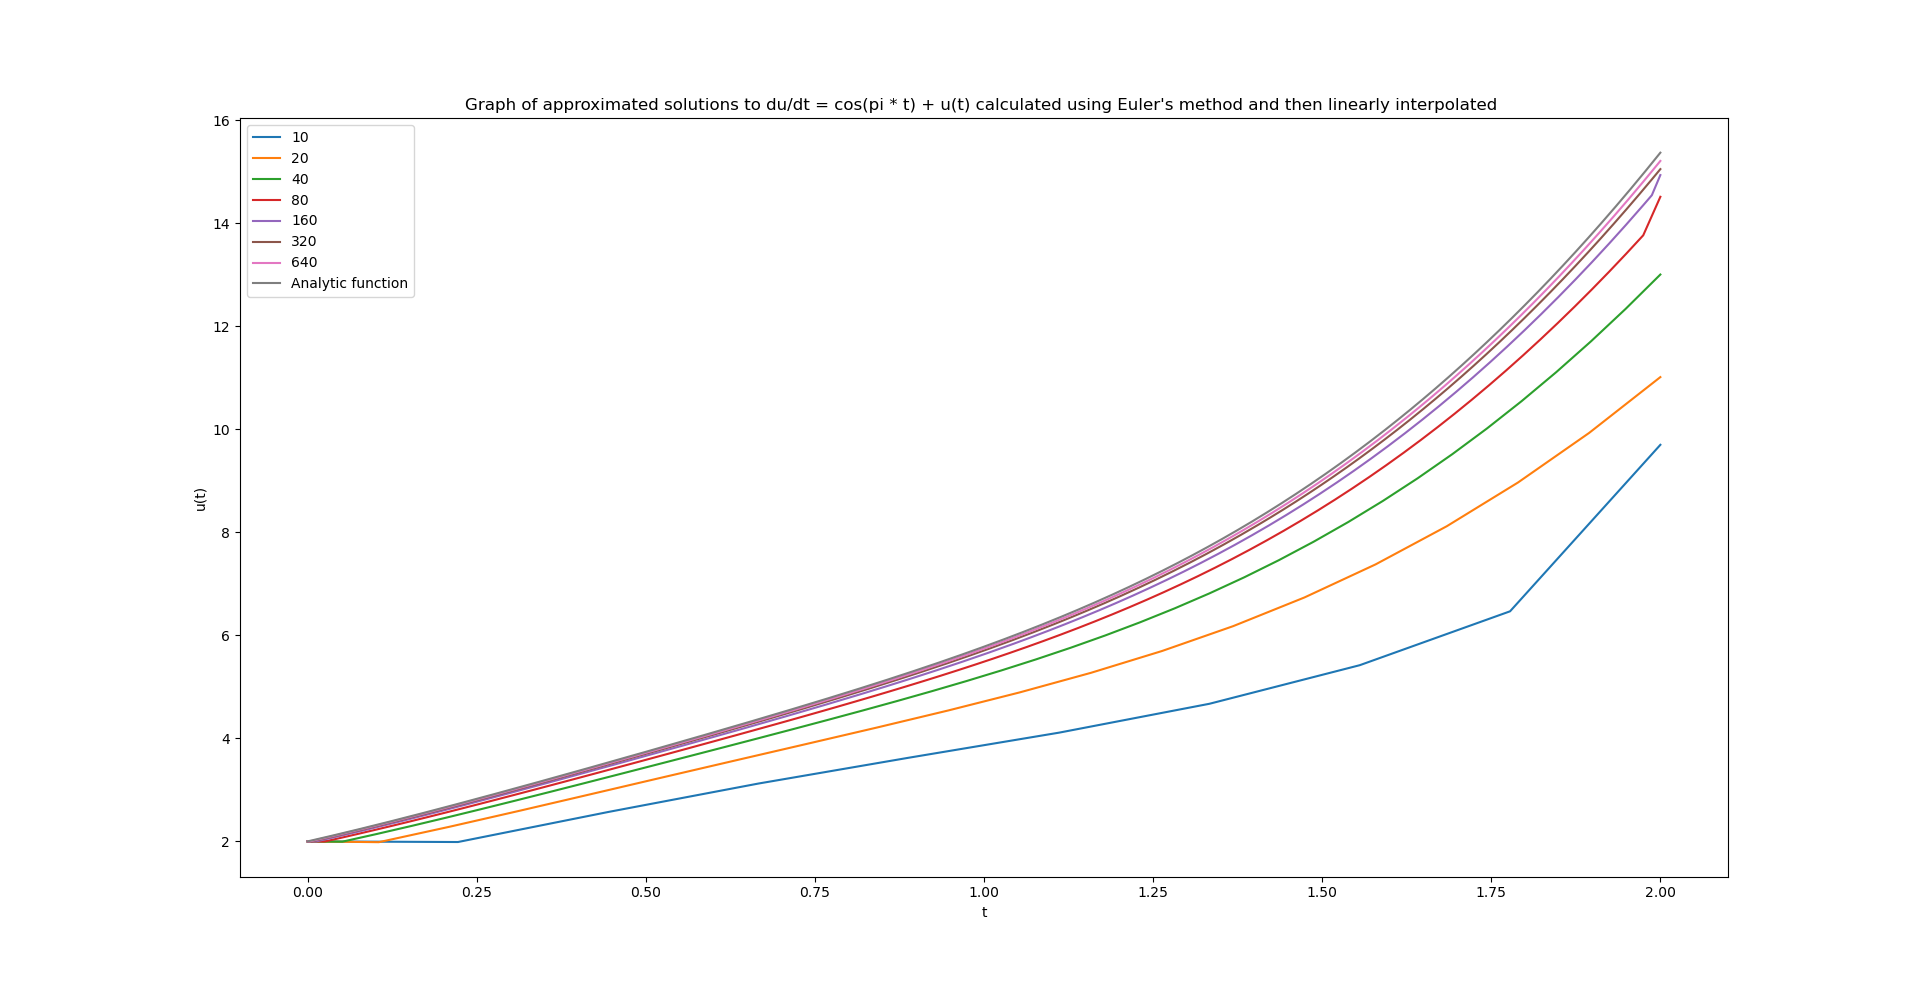
\includegraphics[angle=0,height=10cm]{./img/euler_function.png}
\end{center}

\begin{center}
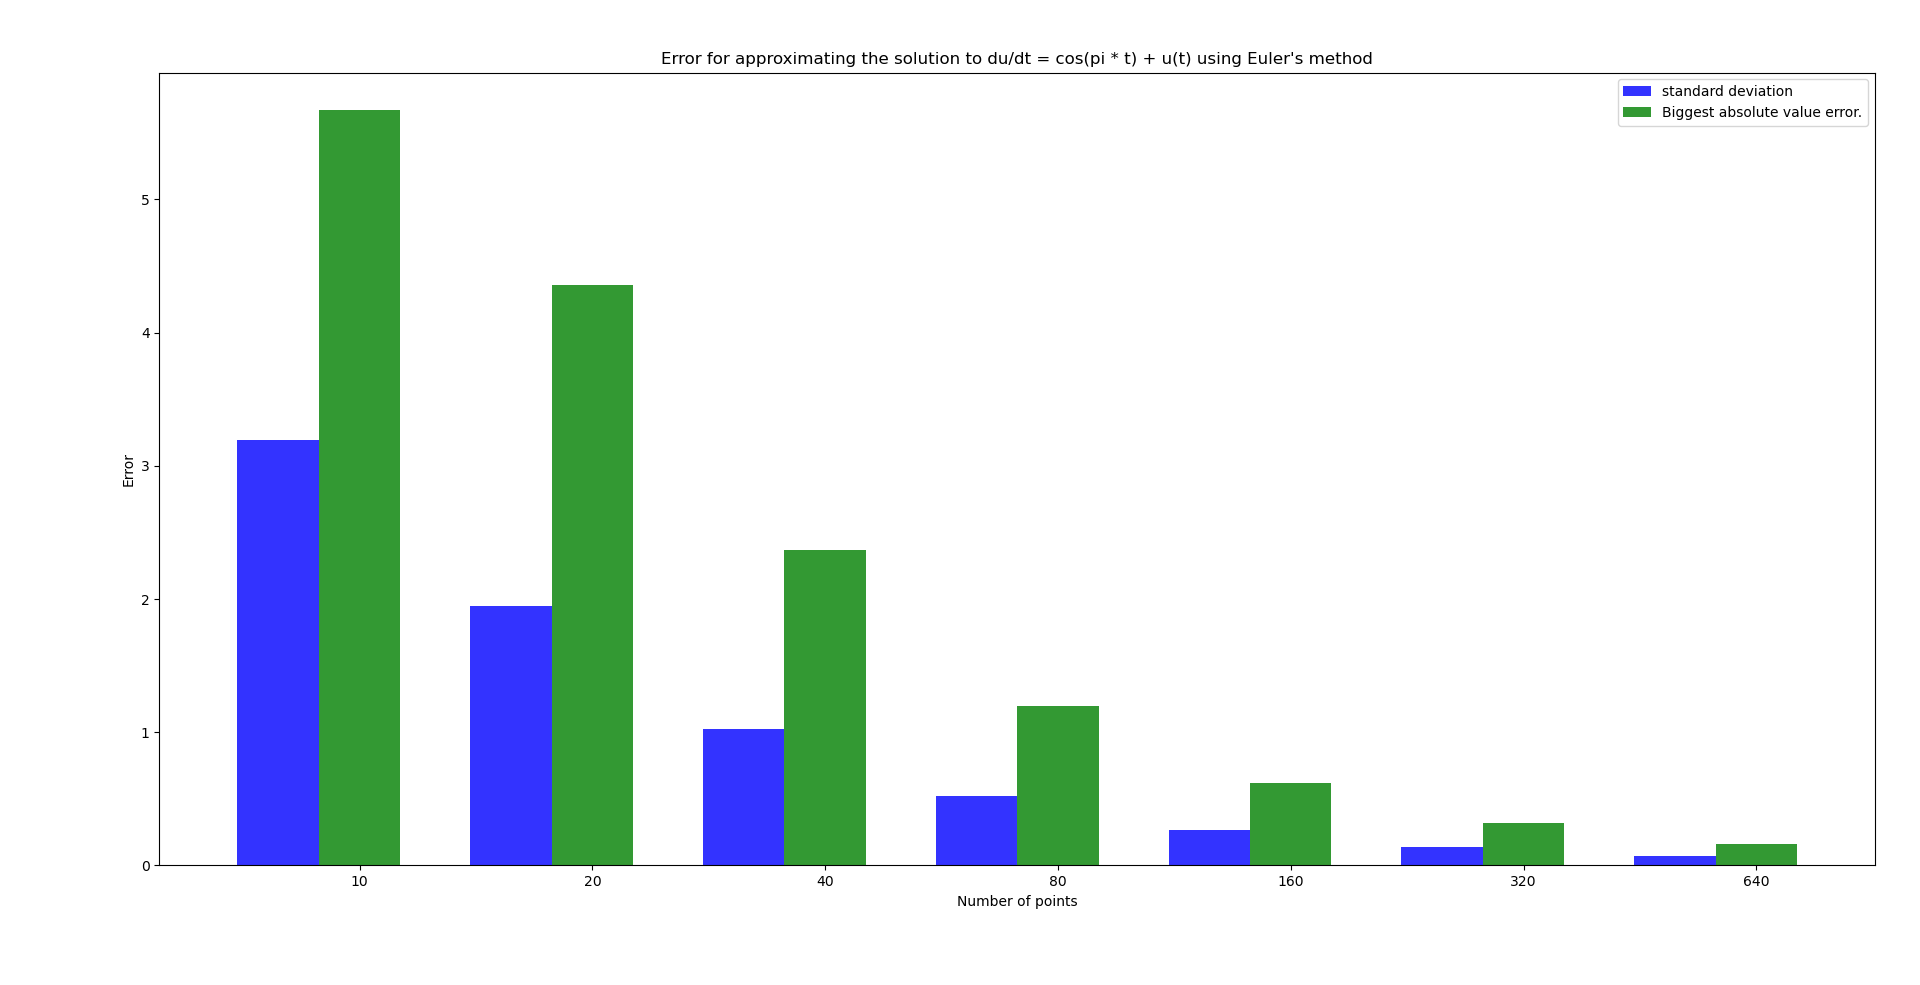
\includegraphics[angle=0,height=10cm]{./img/euler_error.png}
\end{center}


\subsection{2nd order Runge Kutta}
\label{sec:orgde5ffa8}

\begin{center}
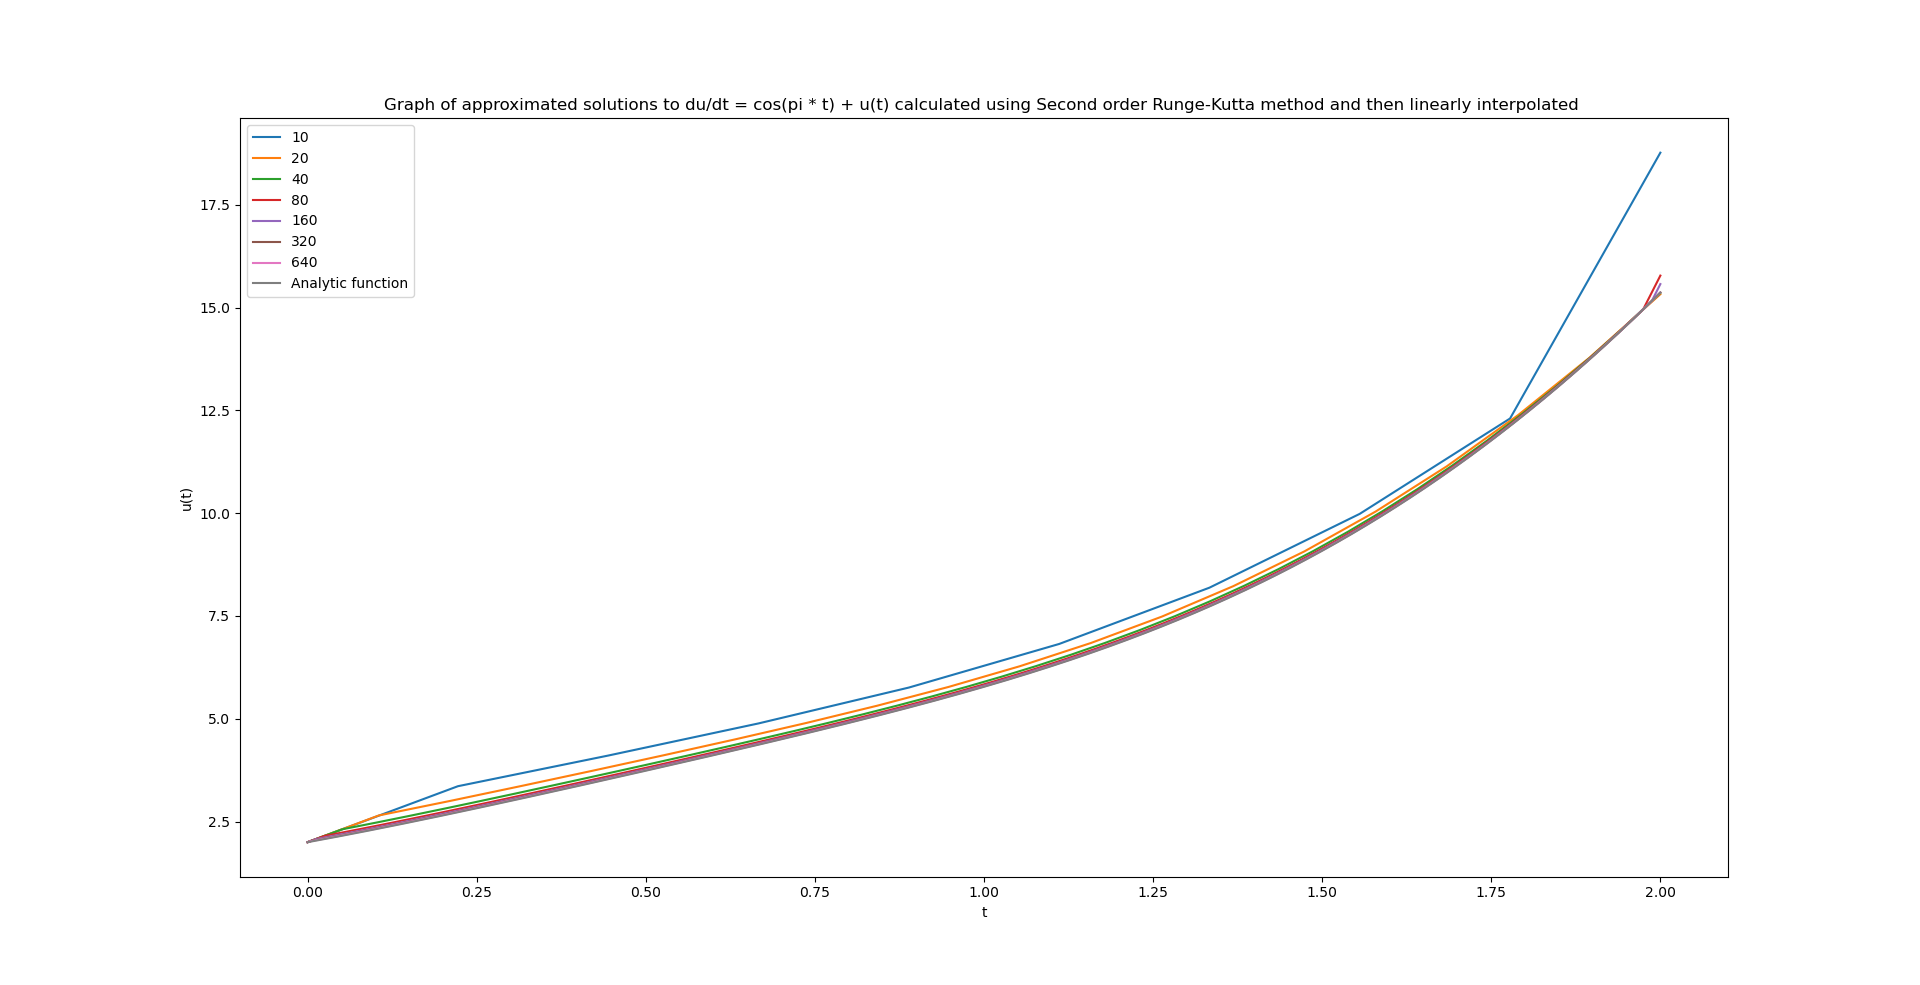
\includegraphics[angle=0,height=10cm]{./img/runge_2_function.png}
\end{center}

\begin{center}
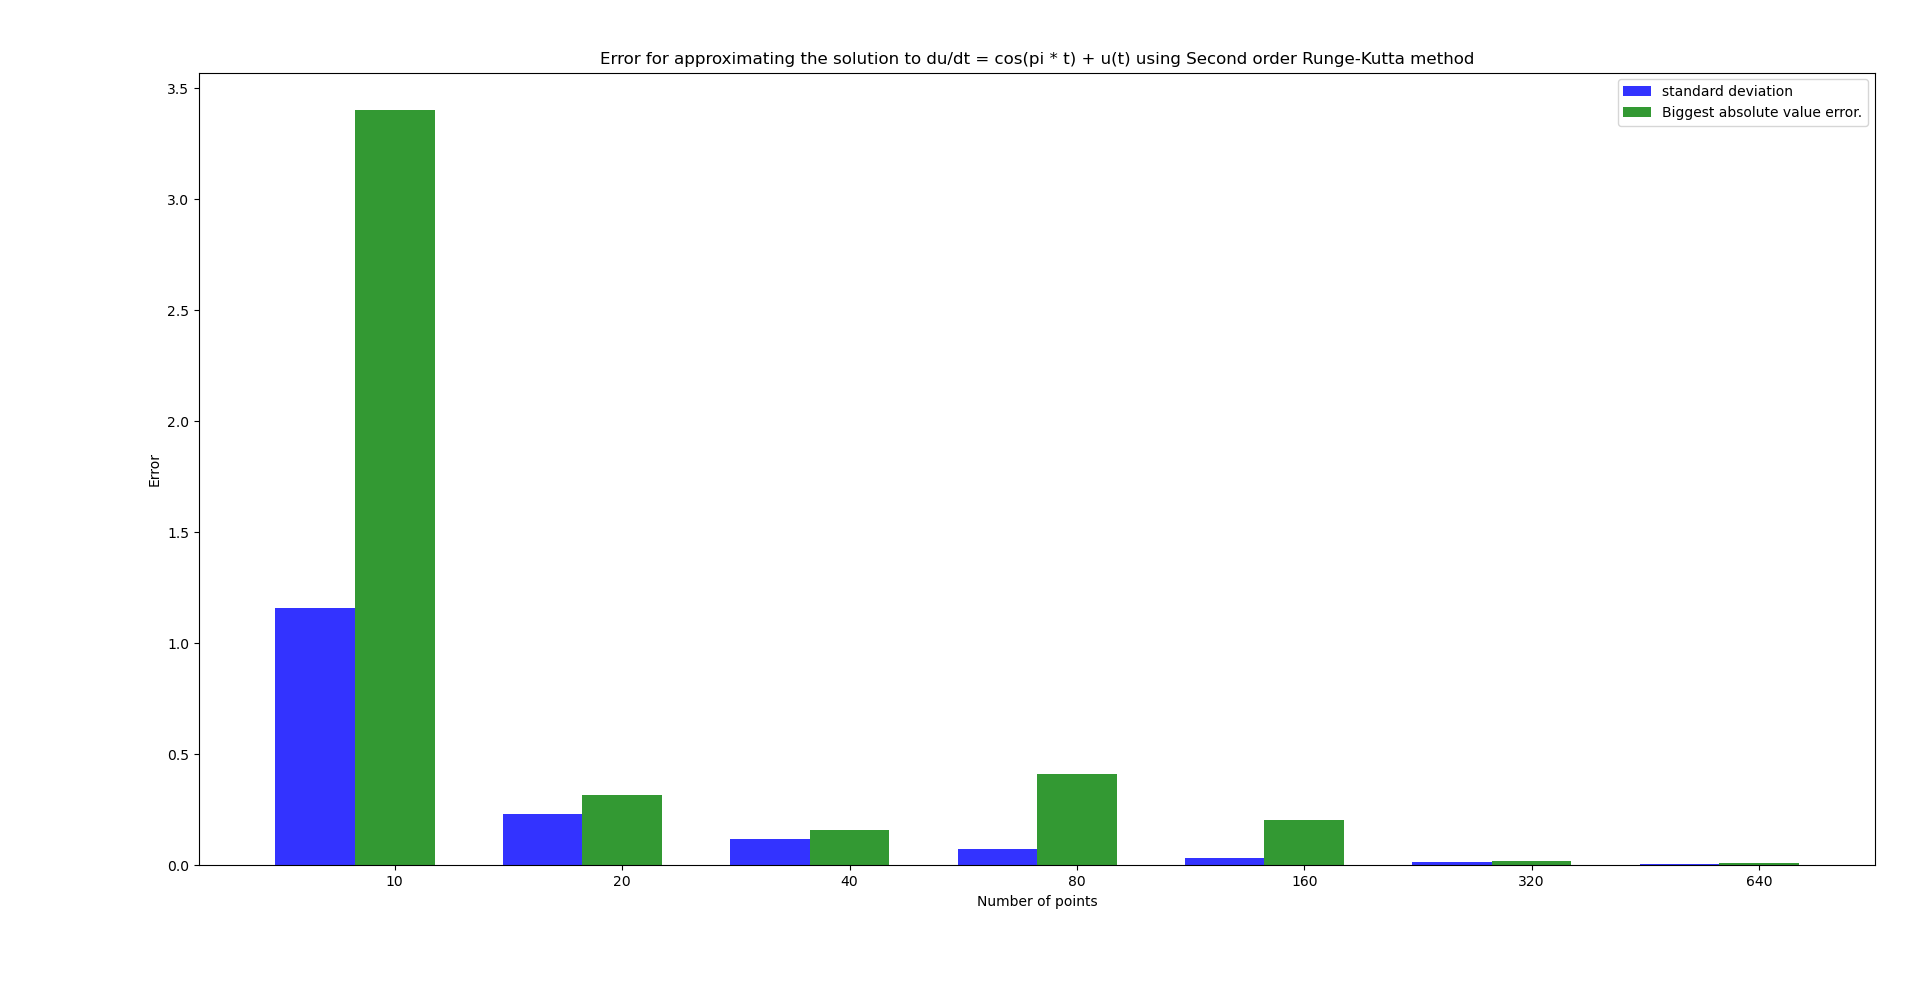
\includegraphics[angle=0,height=10cm]{./img/runge_2_error.png}
\end{center}




\subsection{4th order Runge Kutta}
\label{sec:orga9452c8}

\begin{center}
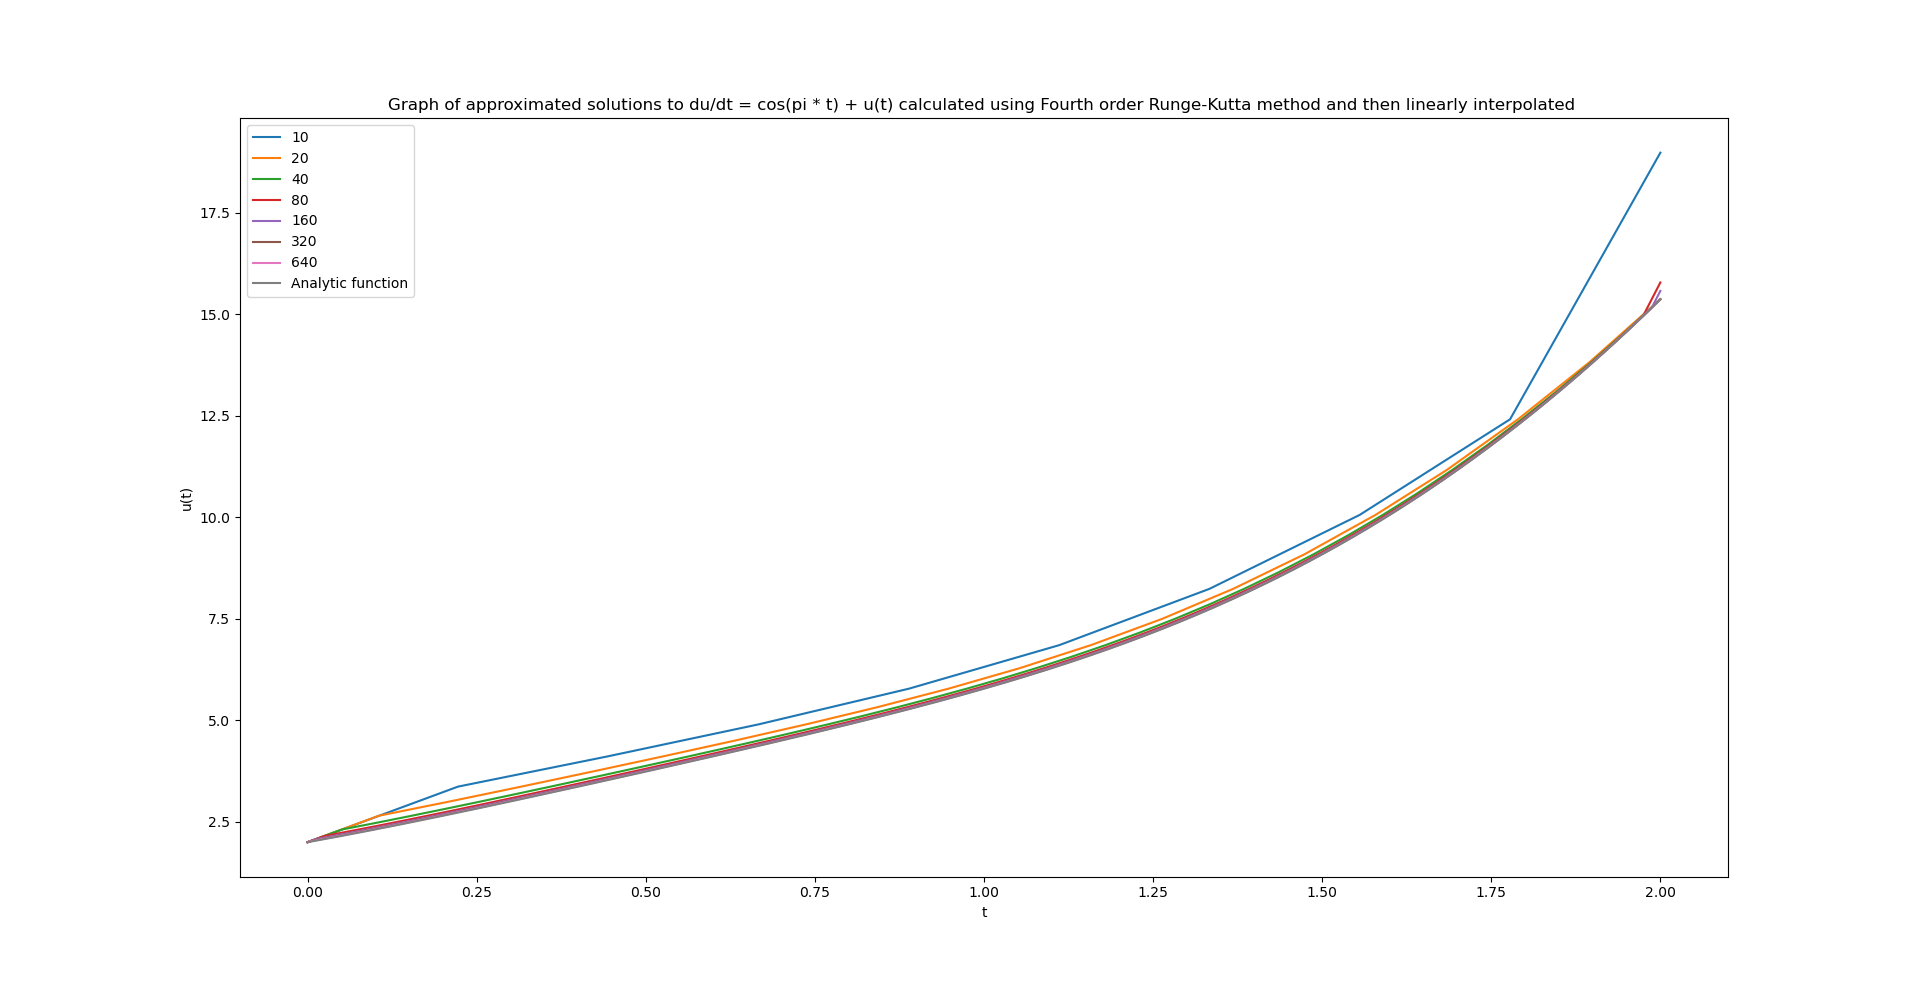
\includegraphics[angle=0,height=10cm]{./img/runge_4_function.png}
\end{center}

\begin{center}
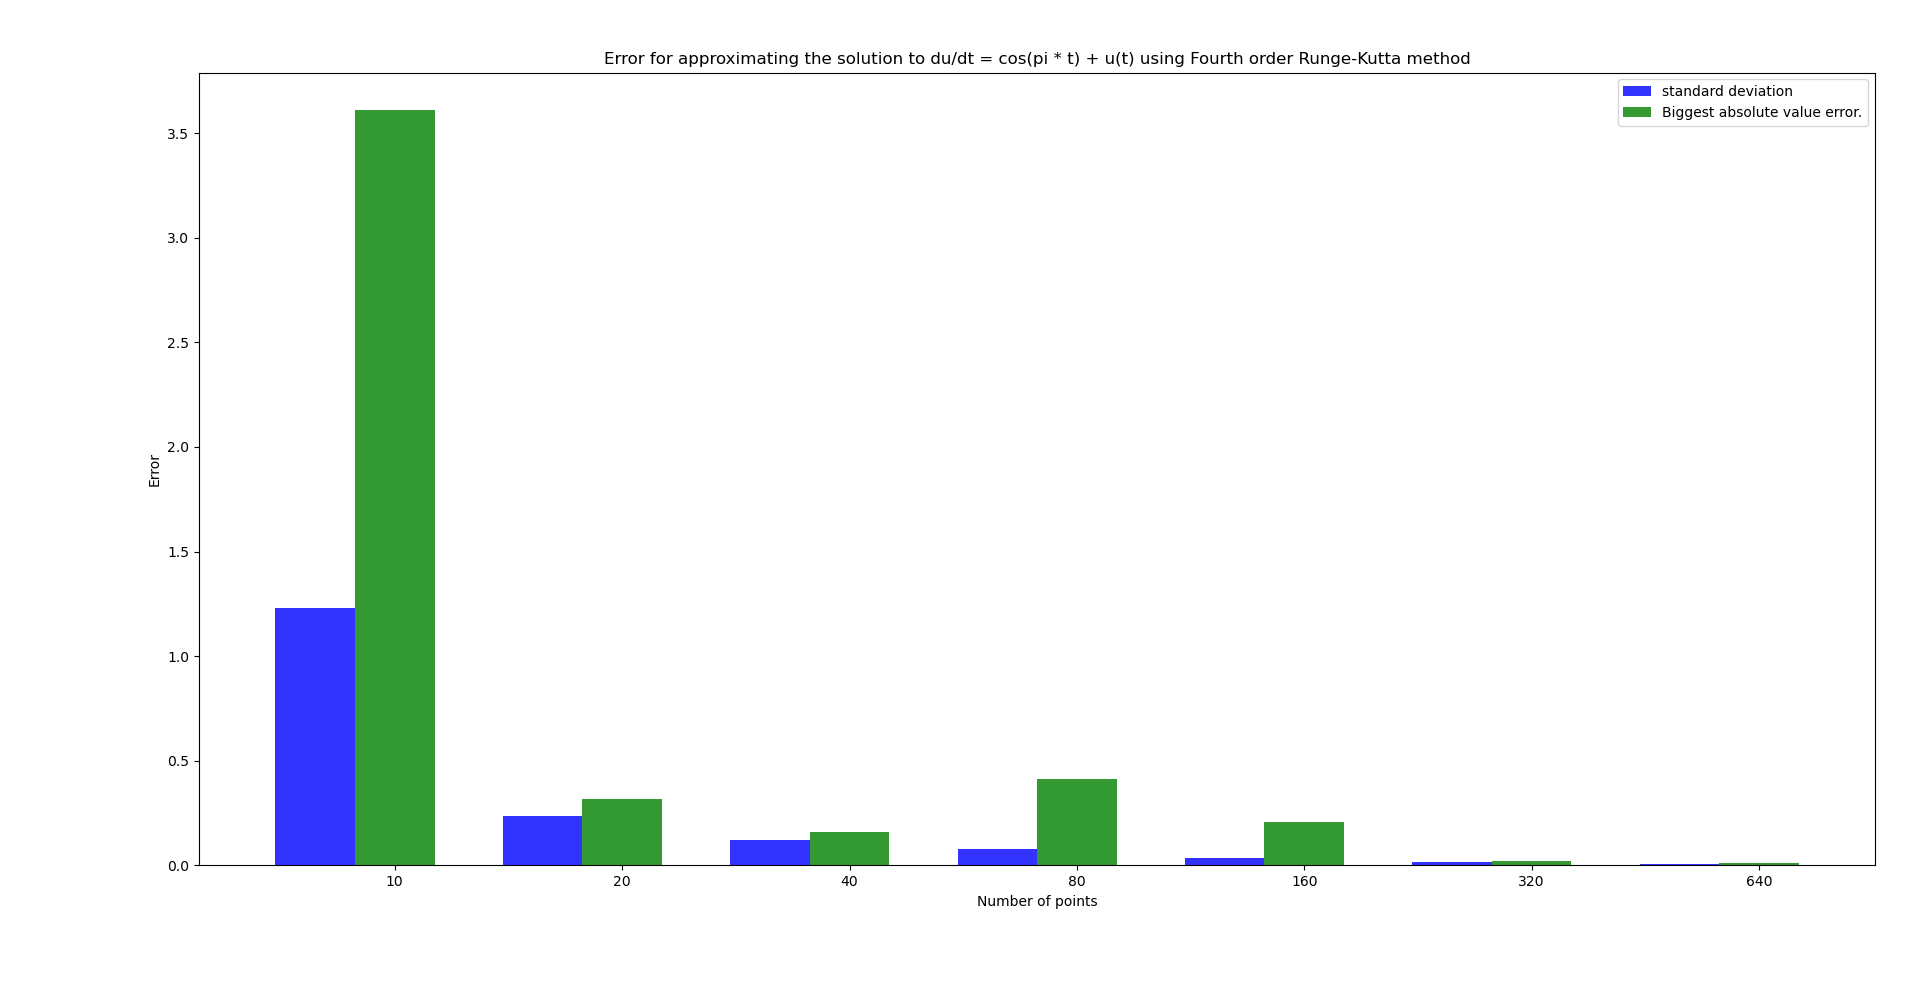
\includegraphics[angle=0,height=10cm]{./img/runge_4_error.png}
\end{center}




\subsection{Adam-Bashforth method}
\label{sec:orge87f3e1}

\begin{center}
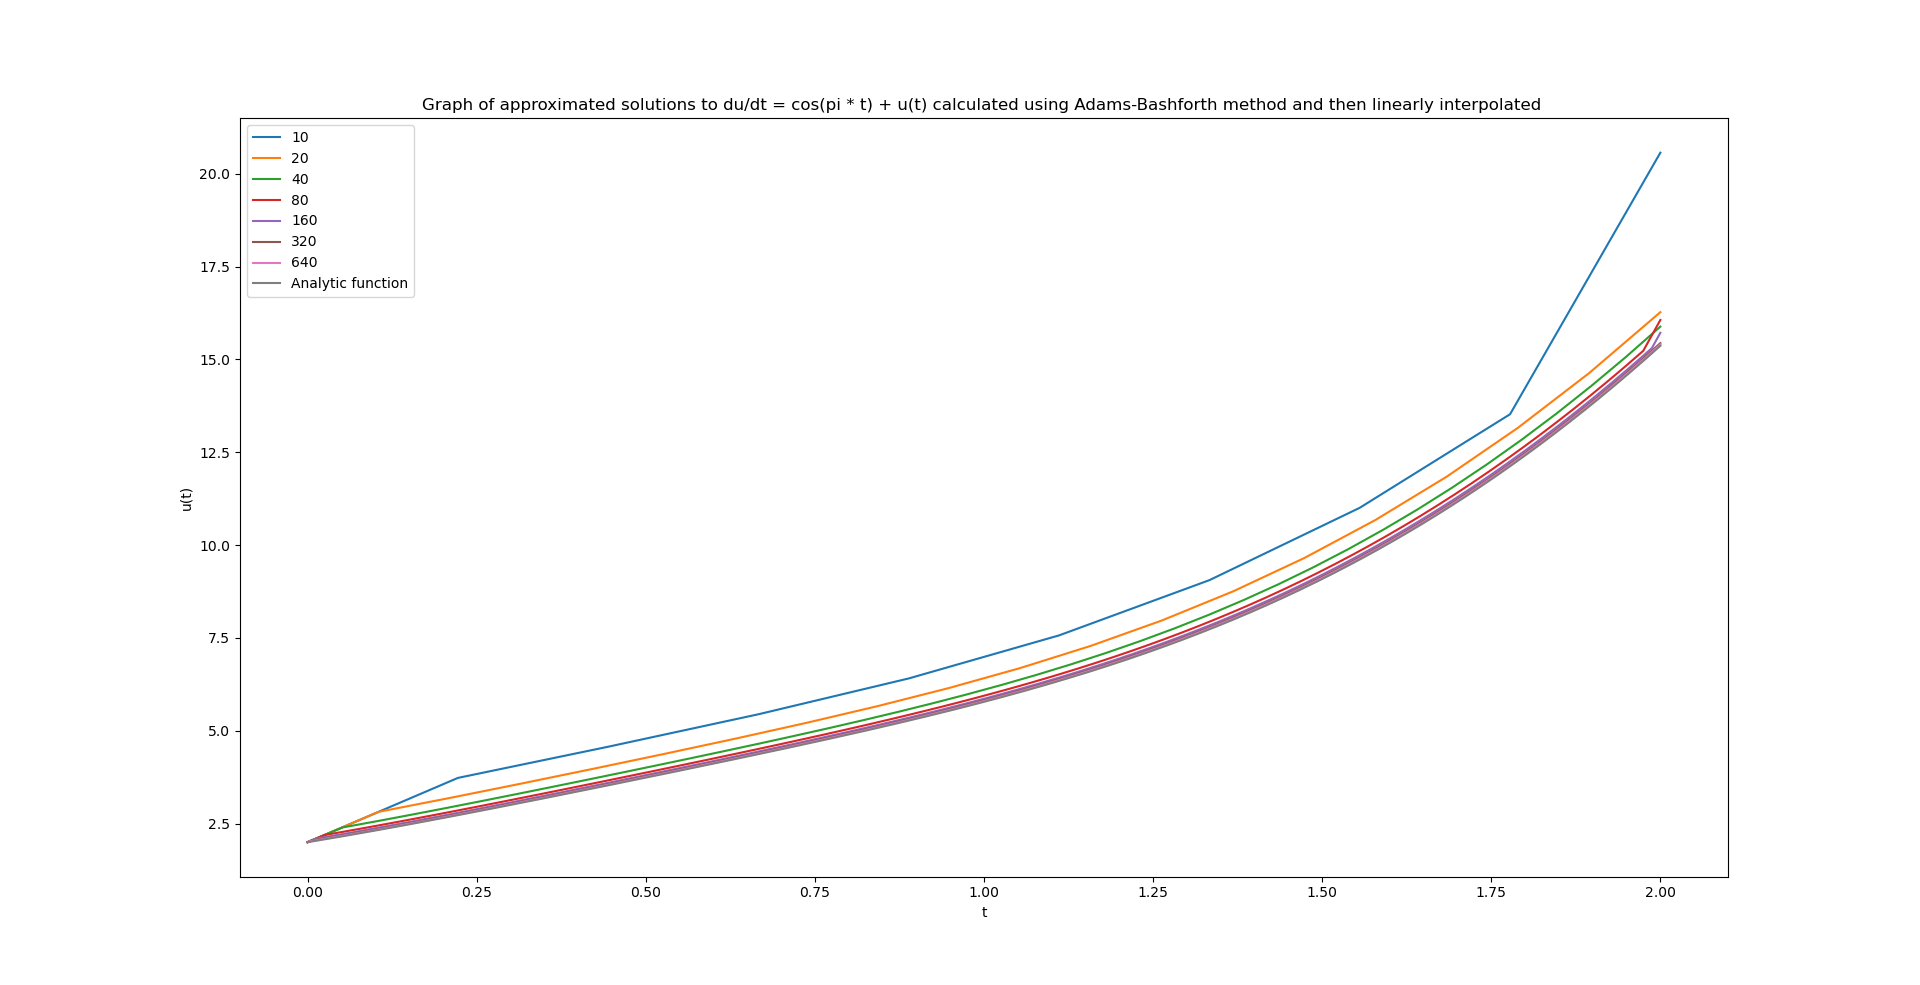
\includegraphics[angle=0,height=10cm]{./img/adam_function.png}
\end{center}

\begin{center}
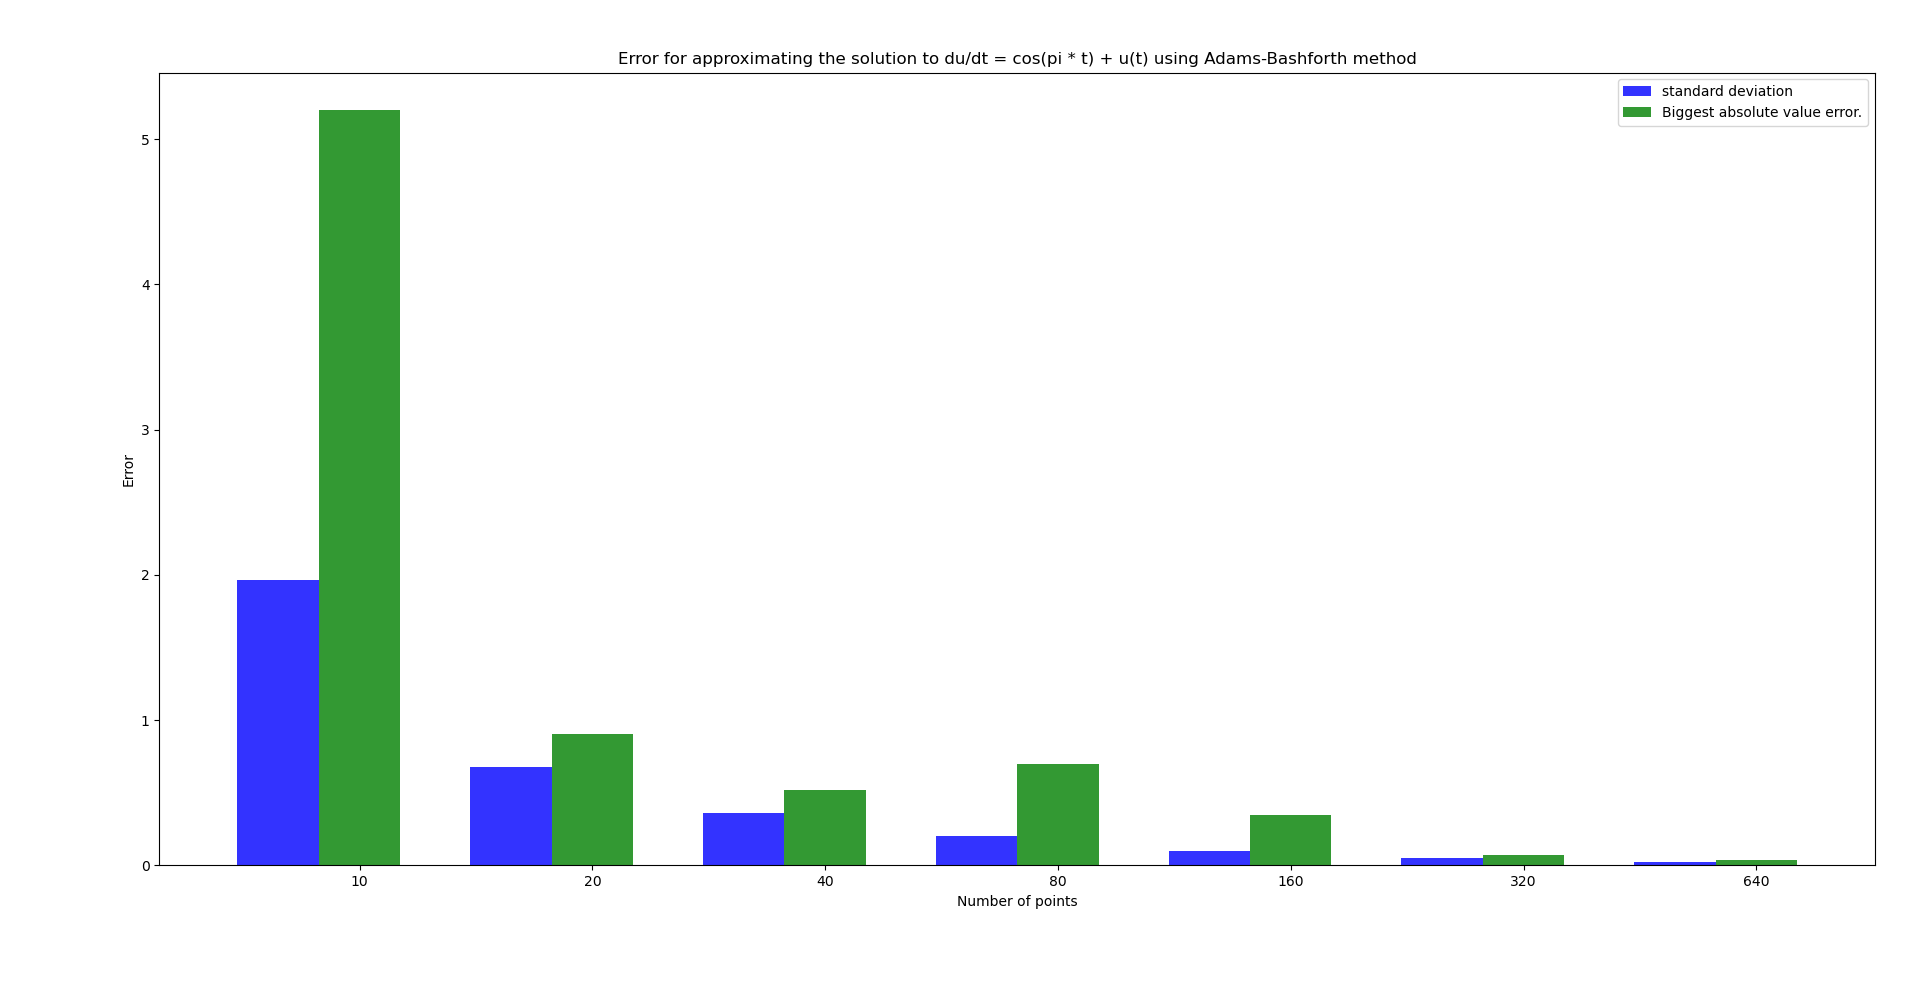
\includegraphics[angle=0,height=10cm]{./img/adam_error.png}
\end{center}

\section{Discussion}
\label{sec:org28e10e5}
\end{document}
